\documentclass[english,10pt]{beamer}
%\usepackage[T1]{fontenc}
%\usepackage[latin9]{inputenc}
\usepackage{mathptmx,amsmath,amssymb,graphicx,bibentry,bbm,babel,ragged2e}
%\usepackage{fontspec}

%\setmainfont{Lucida Grande}
%\setsansfont{Lucida Grande}



\makeatletter

\newcommand{\lyxdot}{.}


 \newenvironment{centercolumns}{\begin{columns}[c]}{\end{columns}}

\usetheme{Warsaw}

\setbeamertemplate{footline}[text line]{}
\setbeamercolor{structure}{fg=purple!50!blue, bg=purple!50!blue}

\setbeamercovered{transparent}


\@ifundefined{showcaptionsetup}{}{%
 \PassOptionsToPackage{caption=false}{subfig}}
\usepackage{subfig}
\makeatother




\begin{document}




\title{Discrete Choice Models for Bike-Sharing Transportation Systems \\ {\small Inference of Discrete-Choice parameters by coupling Statistical Analysis and Agent-based Modeling}}

\author{J.~Raimbault$^{1,2}$}


\institute{$^{1}$Graduate School, Ecole Polytechnique\\
$^{2}$LVMT, Ecole Nationale des Ponts et Chauss{\'e}es\\
}


\date{PIL Presentation - Dpt VET, ENPC \\
under the direction of Z. Christoforou, LVMT, ENPC\\
November 6, 2014}

\frame{\maketitle}


%%%%%%%%%%%%%%%%%%%%
\section{Introduction}
%%%%%%%%%%%%%%%%%%%%

%%%%%%%%%%%%%%%%%
\begin{frame}
\frametitle{Outline}
\tableofcontents{}
\end{frame}
%%%%%%%%%%%%%%%%%

%%%%%%%%%%%%%%%%%
\frame{\frametitle{Research Question}

User surveys in discrete choice are very expensive, and one often has bad quality data. However possible to cross different data source and methods to improve results robustness, as recent work show  \cite{crabtree2012modelling}.
\vfill
\textbf{Research Question : }\textit{To what extent can we improve the estimation of discrete choice parameters by using user questionnaire data with system dynamics raw data,  and coupling statistical analysis and Agent-Based Modeling ?}


}
%%%%%%%%%%%%%%%%%
\begin{frame}
\frametitle{Why study bike-sharing systems ?}
\begin{justify}
\vfill{}

\begin{itemize}
{\justify \item Quick development across the world since 2000, starting from Europe (\cite{demaio2009bike}).}
\vfill{}
{\justify\item Around 200 systems in the world. Ecological and compatible (``sustainable'') transport mode (\cite{o2013mining}).}
\vfill{}
{\justify\item Extensions to unexpected places ? USA (\cite{gifford2004will}) where car is dominant, or China (\cite{liu2012solving}) where relation to bikes has strongly changed these last years.}
\vfill

\item Already well studied : statistical models (\cite{borgnat2009studying,borgnat2009modelisation},\cite{michau2011peut})
or data-mining analysis (\cite{o2013mining},\cite{vogel2011understanding,kaltenbrunner2010urban})
\end{itemize}
\vfill{}
\end{justify}

\end{frame}
%%%%%%%%%%%%%%%%%%%%%%%%%%%%

%%%%%%%%%%%%%%%%%%%%%%%%%%%%
\frame{\frametitle{But Intrinsically non-performant systems...}
\begin{figure}

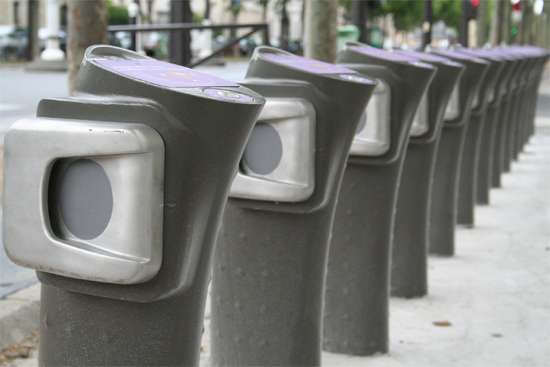
\includegraphics[scale=0.29]{/Users/Juste/Documents/ComplexSystems/CityBikes/Data/images/velib-station-vide}\,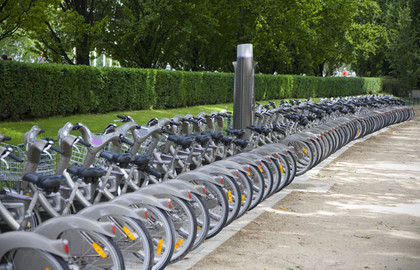
\includegraphics[scale=0.39]{/Users/Juste/Documents/ComplexSystems/CityBikes/Data/images/velibpleine}\caption{Full or empty docking stations in Paris: decrease in the level of
service (source www.velib.paris.fr)}
\end{figure}
}

%%%%%%%%%%%%%%%%%%%%%%%%%%%%

%%%%%%%%%%%%%%%%%%%%%%%%%%%%
\frame{\frametitle{Discrete Choices}
\begin{itemize}
\item Discrete Choice Modeling : theoretical and practical framework to formalize user choice (used in transportation, marketing, politics) \cite{ben1999discrete}, in fact supervised learning with particular loss function)
\vfill
\item Ergonomic tools to estimate models  \cite{bierlaire2006biogeme}
\vfill
\item Bike-sharing studied from this point of view only for modal choice ; should be a good tool to improve knowledge on system and better design or manage it.
\end{itemize}
}

%%%%%%%%%%%%%%%%%%%%%%%%%%%%

%%%%%%%%%%%%%%%%%%%%%%%%%%%%
\begin{frame}
\frametitle{Project Description}

Sequence of Problematics :
\begin{enumerate}
\item Conceive and realize a precise survey to estimate discrete choice models.
\item Problem with Questionnaire administration : how to use this poor quality data ?
\item On the other hand, data available on raw dynamics but also incomplete. 
\item Proposition of indirect inference of DC Parameters by coupling approaches. Core results  more methodological than practical.
\end{enumerate}

\end{frame}


%%%%%%%%%%%%%%%%%%%%
\section{Data Collection}
%%%%%%%%%%%%%%%%%%%%




%%%%%%%%%%%%%%%%%%%%%%%
\frame{
\frametitle{Discrete Choice Questionnaire}

\begin{itemize}
\item Generic web-application for questionnaire administration
\vfill
\item Php server-side application, with standard SQL database
\vfill
\item Direct Biogeme export (specification file with format [BIOGEME\_VARIABLE\_NAME ; BASE\_VARIABLE\_NAME ; BASE\_VALUE ])
\vfill
\item Demo at http://37.187.242.99/Questionnaire

\end{itemize}
}
%%%%%%%%%%%%%%%%%%%%%%%%%%%%

%%%%%%%%%%%%%%%%%%%%%%%%%%%%
\frame{\frametitle{Generic Database}
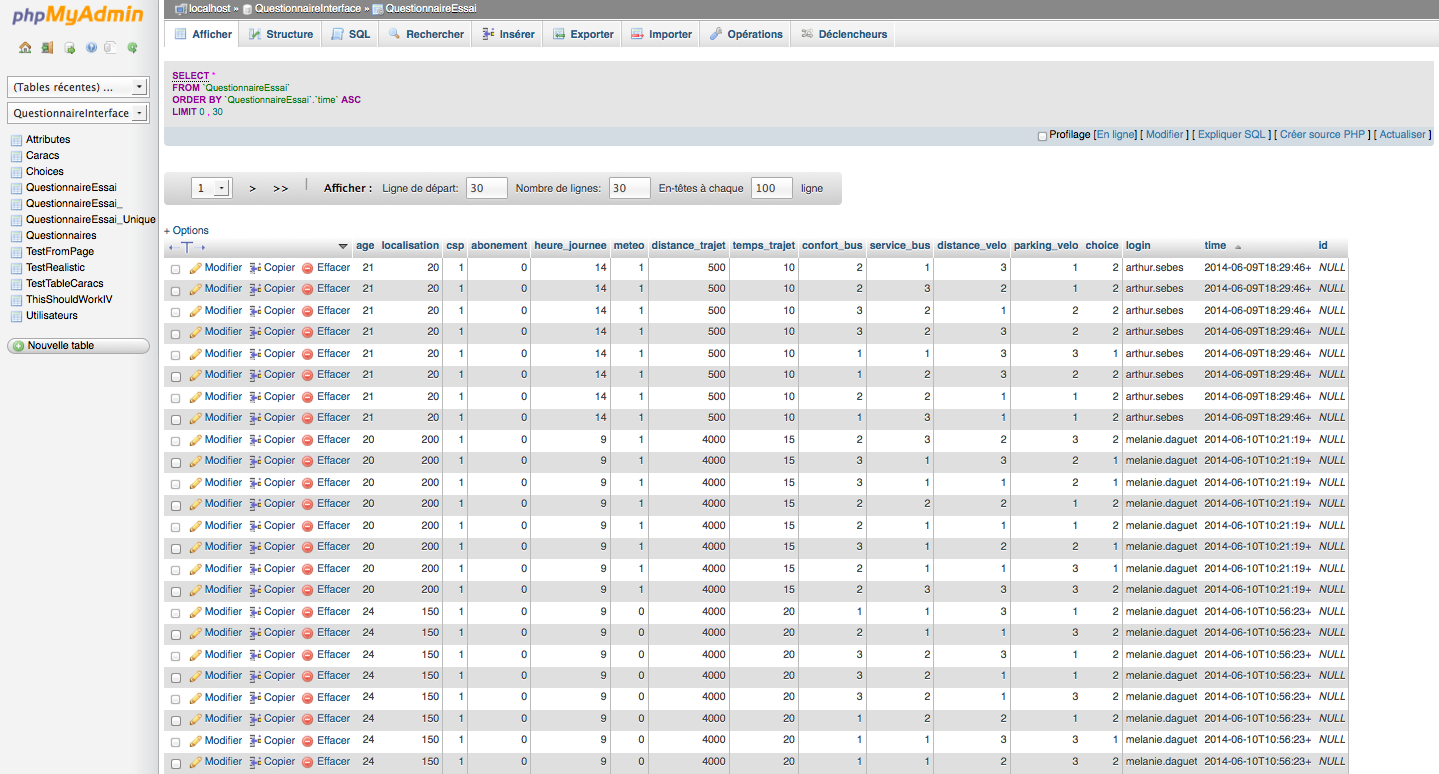
\includegraphics[scale=0.2]{/Users/Juste/Documents/Cours/EconoChoixDiscrets/Project/Docs/Report/screenBase}


}

%%%%%%%%%%%%%%%%%%%%%%%
\begin{frame}
\frametitle{Raw Data : why Open Data ?}

\begin{itemize}
\item Public data provided by the operator in real time. Problem: need a
constantly running collection data process, and only docking station
status (incomplete data).
\vfill{}
\item Why not ask full travel data to operator ? Independent and open research
(\cite{banos2013HDR} ), reporting bias (in \cite{nair2013large}
results are not presented complete because company did not want for
commercial reasons). We do a compromise, and see if we can however
have good results.
\vfill{}
\item Also risk of unconscious spin in the description of results \cite{boutron2010reporting}.
\end{itemize}
\vfill{}
\end{frame}


%%%%%%%%%%%%%%%%%%%%%%%
\begin{frame}
\frametitle{Raw Data collection Process}
\hfill{}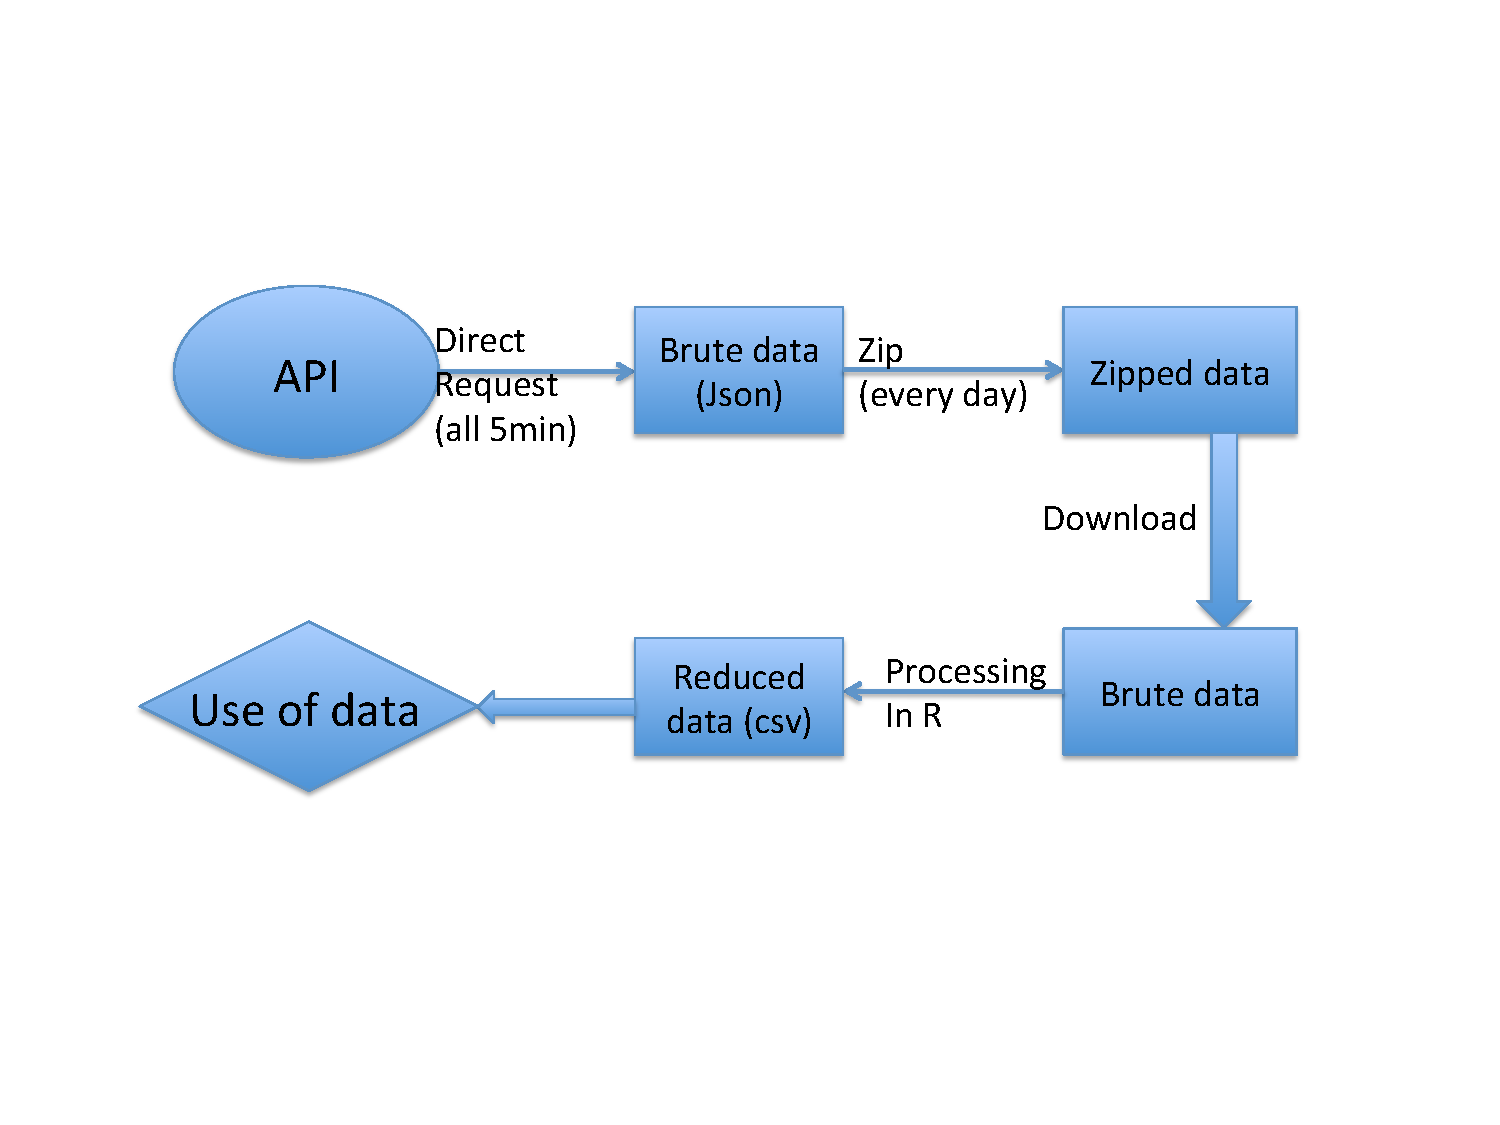
\includegraphics[bb=0bp 100bp 720bp 540bp,scale=0.45]{/Users/Juste/Documents/ComplexSystems/CityBikes/Docs/Stats/data}\hfill{}
\end{frame}


%%%%%%%%%%%%%%%%%%%%
\section{Discrete Choice Modeling}
%%%%%%%%%%%%%%%%%%%%

%%%%%%%%%%%%%%%%%%%%
\frame{\frametitle{Precise Discrete Choice Questionnaire}
\hfill
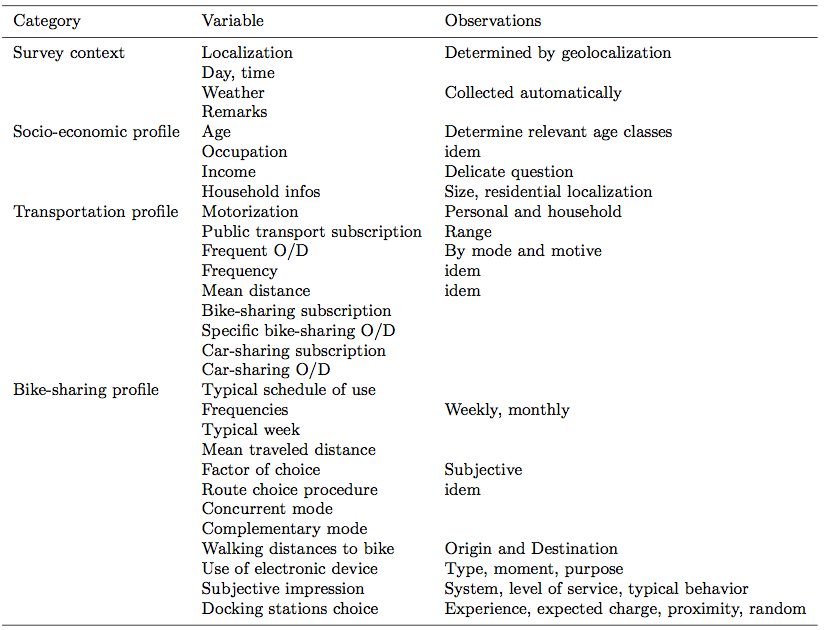
\includegraphics[scale=0.27]{DCQuestionnaire}
\hfill \hfill
}
%%%%%%%%%%%%%%%%%%%%%%%%%%%%

%%%%%%%%%%%%%%%%%%%%%%%%%%%%
\frame{\frametitle{Simplified Discrete Choice Model}
\itemize{

\item Stated preference model, Conception and estimation in \cite{bourcet2014vlib} 

\item Variables :
\begin{itemize}
\item age
\item professional categorization
\item regular user
\item average distance to public transport
\end{itemize}

\item Choice of mode between bus and bike-sharing, with attributes : travel distance $D$, expected travel time $t$, time to find a bike $t_B$, time to drop a bike $t_D$, bus delay $D$ and bus comfort $C$ (3 discretization levels).

\item Utilities : $U_{bus}=\sum{\beta_{X_{bus}}X_{bus}}+\varepsilon_1$ and $U_{bike}=\sum{\beta_{X_{bike}}X_{bike}}+\varepsilon_2$.

\item Results : $\beta_D \in [-0.06,0]$ and $\beta_{t_{B}}\in [-0.25,-0.15]$
}

}


%%%%%%%%%%%%%%%%%%%%
\section{Statistical Analysis}
%%%%%%%%%%%%%%%%%%%%


\frame{\frametitle{A case study on missing data}
Many methods to fill incomplete data \cite{rubin2009multiple}.
Case study of comparison between two proposed in  \cite{crowe2010comparison} and  \cite{mitra2010comparison}.
\bigskip
\bigskip

Main conclusions :
\begin{itemize}
\item Deleting rows with missing variables leads to less bias but more variance
\item Use heuristic to know if complete before or after computing outputs (parameters of generalized estimator).
\end{itemize}
}


%%%%%%%%%%%%%%%%%%
\frame{\frametitle{Data-mining for dimensionality reduction}
\begin{figure}
\label{fig:info}
\centering
\subfloat[Clustering coefficient as a function of cluster number for different
values of sampling step.]{\includegraphics[scale=0.22]{/Users/Juste/Documents/ComplexSystems/CityBikes/Results/Clustering/clusterNumber}}
\hfill{}\subfloat[Plot of the value of the clustering coefficient for k=2 (red) and
k=3 (green), as a function of sampling step.]
{\includegraphics[scale=0.26]{/Users/Juste/Documents/ComplexSystems/CityBikes/Results/Clustering/infoLoss}}
\caption{Influence of sampling interval on quantity of conserved information
in the clustering process.}
\end{figure}

}
%%%%%%%%%%%%%%%%%%%


%%%%%%%%%%%%%%%%
\frame{\frametitle{Inference of OD Fields}

\vfill{}

Core of the parametrization : estimation of O/D fields with gaussian
kernels non-parametric estimation (\cite{tsybakov2004introduction})
with package kernlab (\cite{karatzoglou2004kernlab}). With $(d_{i}(t))$
real arrivals at $(\vec{x}_{i}(t))$, $D(t)$ spatial field is given
by
\[
[D(t)](\vec{x})=\frac{1}{K}\sum_{i}d_{i}(t)\cdot exp(\frac{\left\Vert \vec{x}-\vec{x}_{i}\right\Vert }{2\sigma^{2}})
\]
Similar to Geographically Weighted Regression Methods \cite{brunsdon1998geographically},\cite{brunsdon2002geographically}

\hfill{}
\includegraphics[scale=0.17]{/Users/Juste/Documents/ComplexSystems/CityBikes/Results/Kernel/example}\hfill{}

}
%%%%%%%%%%%%%%%%%%





%%%%%%%%%%%%%%%%%%%%
\section{Agent-Based modeling}
%%%%%%%%%%%%%%%%%%%%

%%%%%%%%%%%%%%%%%%%%%%%
\frame{\frametitle{Settings and agents}

ABM proposed in  \cite{raimbault2014user}.
\vfill{}

\begin{itemize}
\item Agents: bikers with information $i(b)$ (boolean), tolerated walking
radius $r(b)$ and mean speed $\bar{v}(b)$; docking stations located
in space with current standing bikes $p_{b}(s,t)$ and capacity $c(s)$
\end{itemize}
\vfill{}

\begin{itemize}
\item Euclidian network \textrm{$N=(V,E)$, representing the road network.
Stations are nodes of the network and movement of bikers is embedded
in the trace of $N$ in $\mathbb{R}^{2}$}
\end{itemize}
\vfill{}

\begin{itemize}
\item Scale of the district; we suppose known temporal fields of origin
$O(t)$ and destination $D(t)$ (probabilities of O/D given a trip),
boundaries conditions $N(t)$ as flows (in- and outflows) at fixed
boundaries points
\end{itemize}
\vfill{}

}

%%%%%%%%%%%%%%%%%%%%%%%
\frame{\frametitle{Temporal Evolution}

At each time step:\vfill{}

\begin{itemize}
\item Start new travels randomly using $O,D,N$ \vfill{}

\item Make bikers in travel advance of the corresponding distance \vfill{}

\item Finish travels and redirect bikers when needed (see flowchart of bikers
behavior)
\end{itemize}

}

%%%%%%%%%%%%%%%%%%%%%%%
\frame{\frametitle{Bikers behavior}

\hfill{}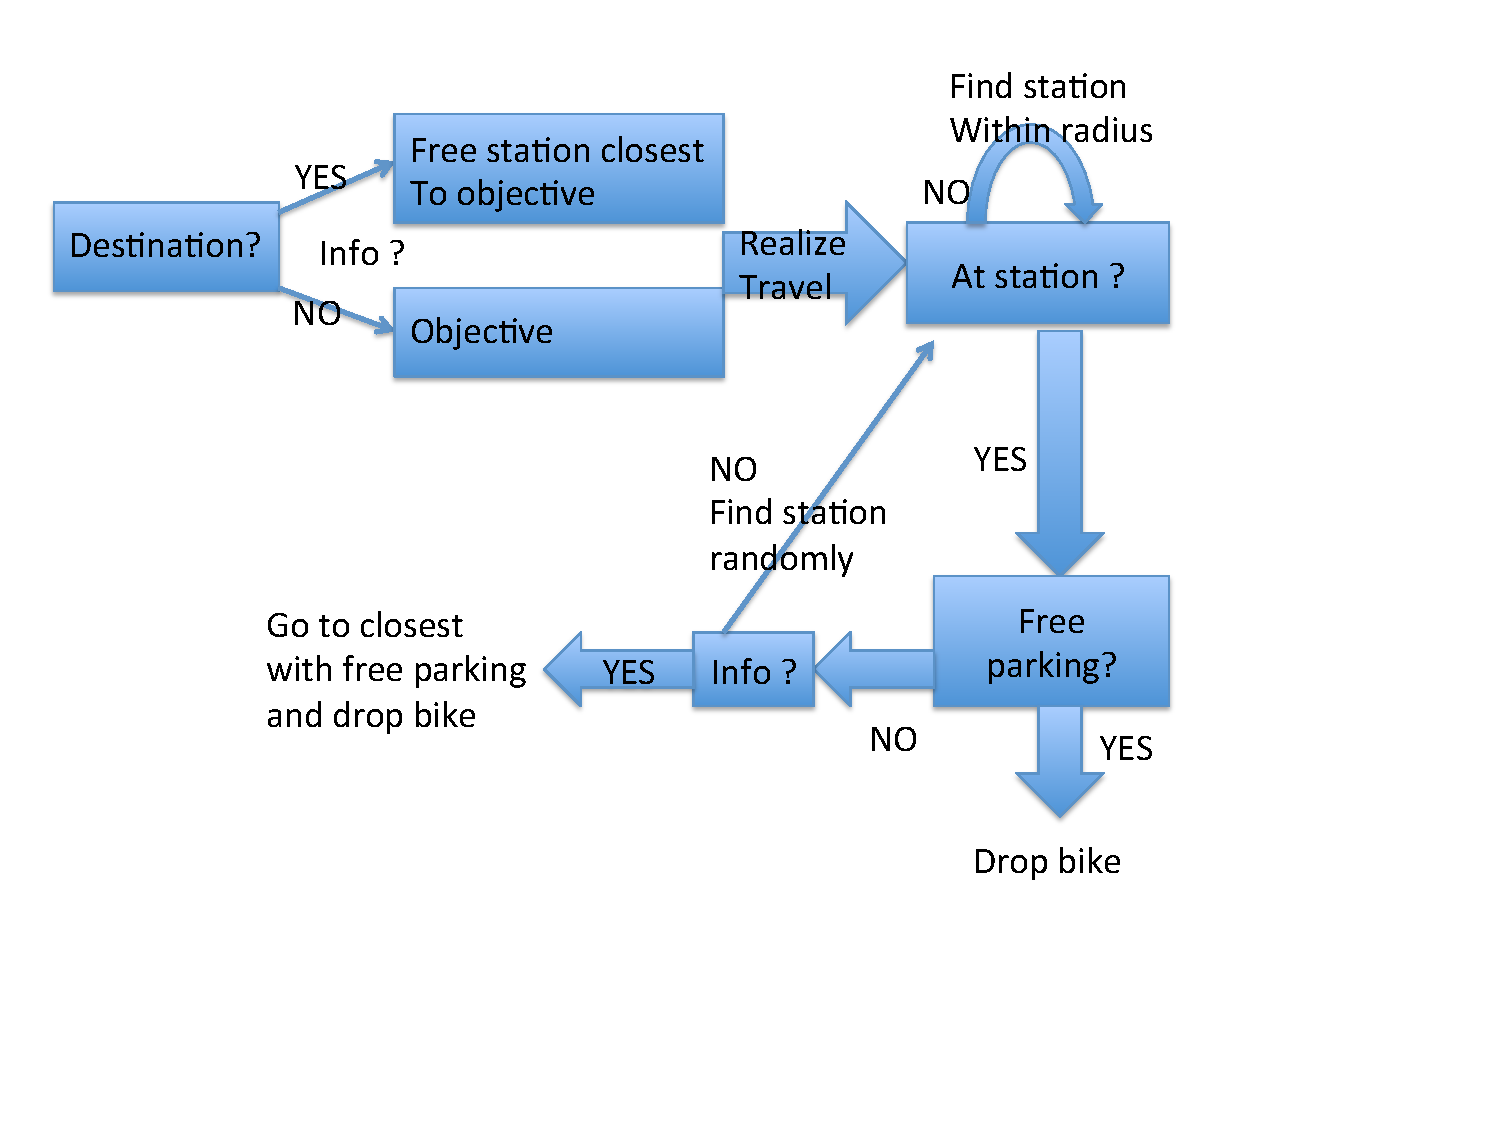
\includegraphics[scale=0.4]{/Users/Juste/Documents/ComplexSystems/CityBikes/Docs/ABM/flowchart}\hfill{}
}


%%%%%%%%%%%%%%%%%
\frame{\frametitle{Discrete Choice in Bikers behavior}

Utilities functions when needs to drop a bike at a full station or take one at an empty one, with $t_w$ average waiting time and $\tilde{d}$ distance to closest station

With information :
\[
U_w(i=1)=\beta_t t_w + \beta_d \tilde{d} + \varepsilon_w
\]
\[
U_m(i=1)=\beta_t \frac{d\textquoteright}{\bar{v}} + \beta_d \tilde{d}\textquoteright + \varepsilon_m
\]

Without information :
\[
U_w(i=0)=\beta_t t_w  + \varepsilon_w
\]
\[
U_m(i=0)=\beta_t \frac{d\textquoteright}{\bar{v}}  + \varepsilon_m
\]
}




%%%%%%%%%%%%%%%%%%%%
\section{Inference of Unknown Parameters}
%%%%%%%%%%%%%%%%%%%%


%%%%%%%%%%%%%%%%%%%%%%%
\frame{\frametitle{Calibration Procedure}
Calibration of model on mean MSE on load factors time-series, $E=<E(k)>_k$ with
\[
E(k)=\frac{1}{\left|S\right|\left|T\right|}\sum_{t\in T}\sum_{s\in S}\left(\frac{p_{b}(s,t)}{c(s)}-lf(s,t)\right)^{2}
\]
Parameters :
\begin{itemize}
\item $\bar{r}$ mean walking radius of bikers
\item $p_i$ probability to have information
\item $\sigma$ kernel size for fields inference
\item DC parameters $\beta_t,\beta_d$
\end{itemize}

Parameter Space : Hypercube $\beta_d \in [-0.06,0]$, $\beta_{t}\in [-0.25,-0.15]$, $\bar{r}\in [0,1000],\sigma \in [50,500]$ and $p_i\in [0.3;0.7]$.
}



%%%%%%%%%%%%%%%%%%%%%%%

%%%%%%%%%%%%%%%%%%%%%%%
\frame{\frametitle{Calibration : Results}

On convergent runs (76\%) : $(\bar{r},p_i,\sigma,\beta_t,\beta_d)=(238\pm 51,0.67\pm 0.08,321\pm 69,-0.05 \pm 0.01, -0.16\pm 0.02)$.

\begin{figure}
\label{fig:calib}
\centering
\subfloat[Response surface along $(\sigma,p_i)$ dimensions.]{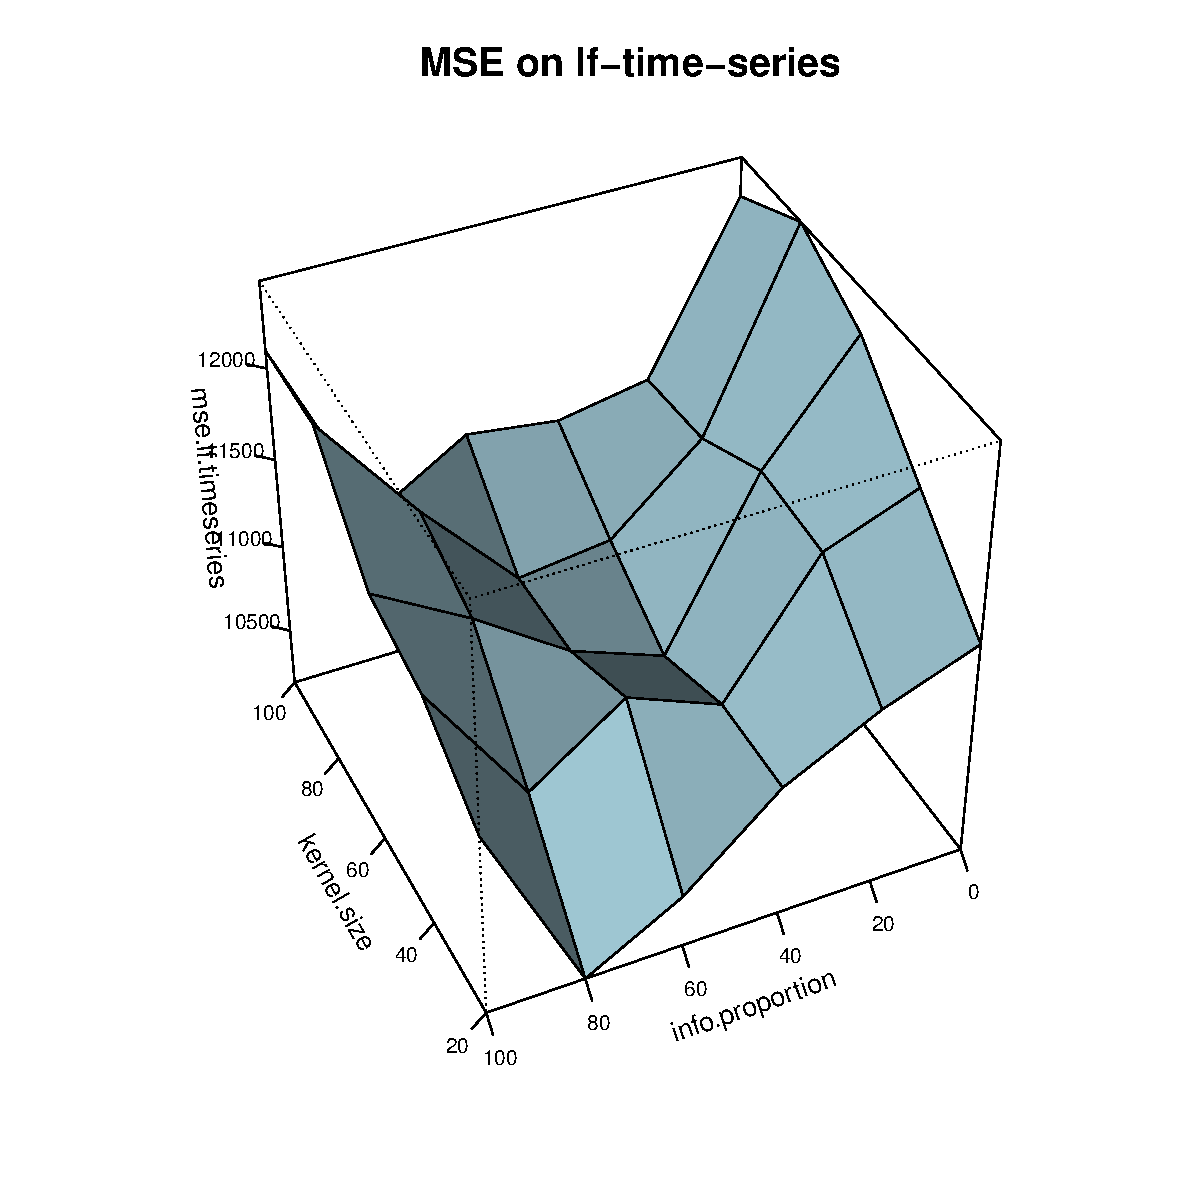
\includegraphics[scale=0.25]{/Users/Juste/Documents/Cours/PIL/DiscreteChoicesBikeSharing/Docs/Report/figures/calib3d}}
\hfill{}\subfloat[Along $(\beta_d,\beta_t)$.]{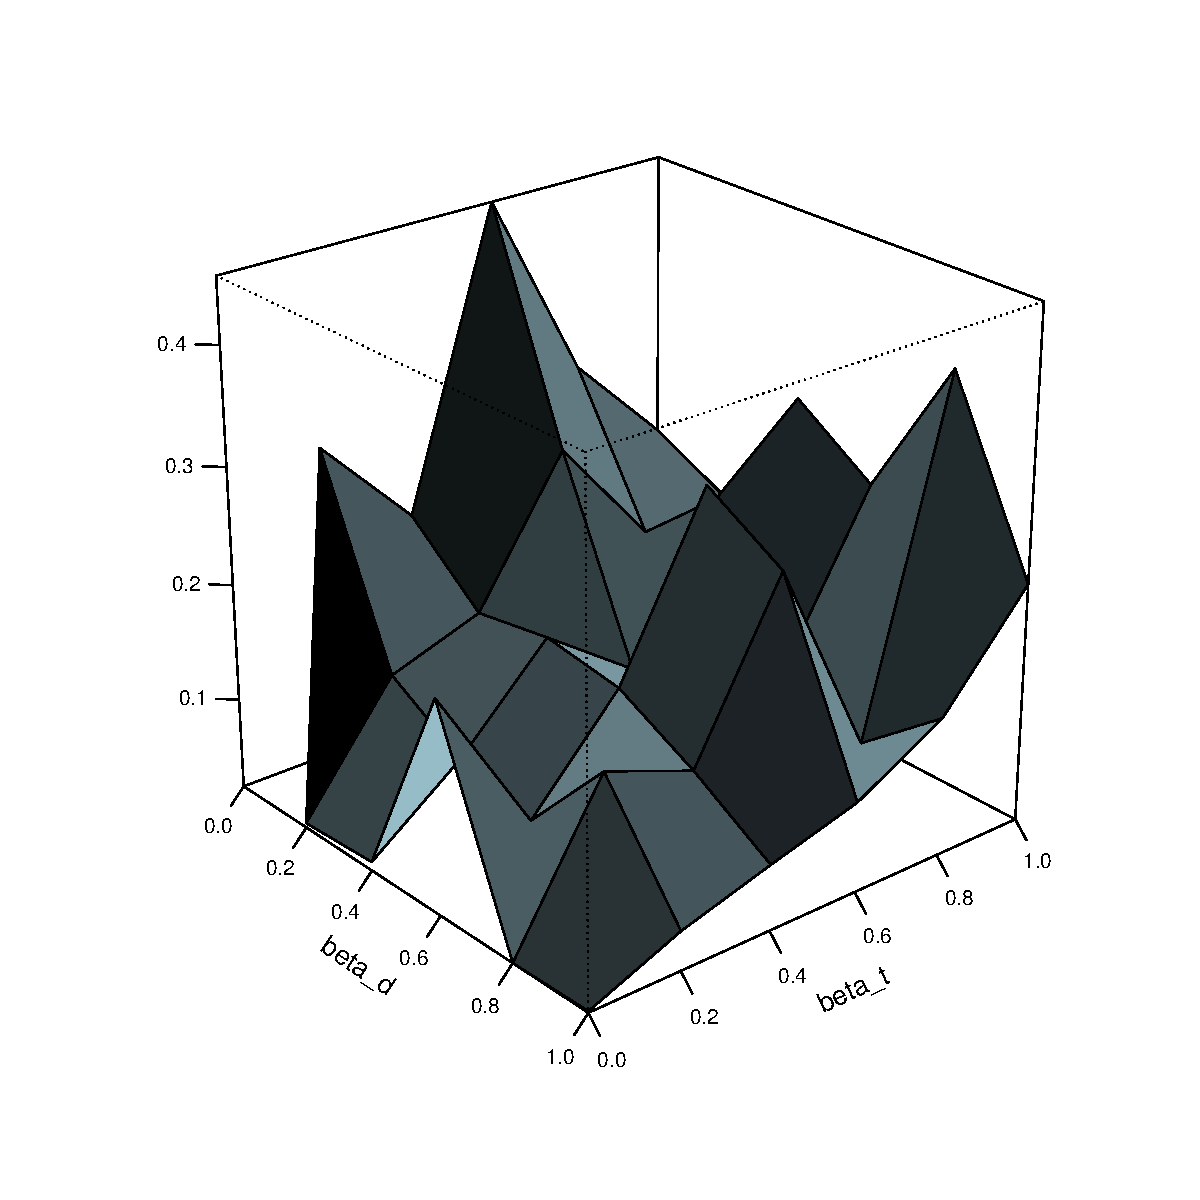
\includegraphics[scale=0.25]{/Users/Juste/Documents/Cours/PIL/DiscreteChoicesBikeSharing/Docs/Report/figures/calib_chaos}}
\caption{Example of Mean-square error response surfaces, obtained with $K=100$ repetitions for each combination of parameters. As some parameters allow a regular, almost convex behavior, ideal for simplex calibration, other give chaotic landscapes.}
\end{figure}

}

%%%%%%%%%%%%%%%%%%%%%%%
\frame{\frametitle{Large Deviations of Gradient Algorithm}
Markov Formalism : Master equation for system State
\[
\partial_{t}P(\mathcal{C},t)=\sum_{\mathcal{C}'\neq\mathcal{C}}W(\mathcal{C}'\rightarrow\mathcal{C})P(\mathcal{C}',t)-r(\mathcal{C})P(\mathcal{C},t)
\]
Large Deviation function with $s$ conjugated with activity $K$: $<e^{-sK}>\sim e^{t\psi(s)}$
$s$-modified dynamic :
\[
\partial_{t}P(\mathcal{C},s,t)=\sum_{\mathcal{C}'\neq\mathcal{C}}W_{s}(\mathcal{C}'\rightarrow\mathcal{C})P(\mathcal{C}',t)-r(\mathcal{C})P(\mathcal{C},t)
\]
that drives the cloning algorithm, equivalent to a Markov dynamic with escape rate $r_{s}(\mathcal{C})=\sum_{\mathcal{C}'\neq\mathcal{C}}W_{s}(\mathcal{C}\rightarrow\mathcal{C}\textquoteright)-r(\mathcal{C})$.

}

%%%%%%%%%%%%%%%%%%%%%%%
\frame{\frametitle{Large Deviations of Gradient Algorithm}

\begin{figure}
\label{fig:cloning}
\subfloat[$\psi(s)$ for $K=20...100$]{\includegraphics[scale=0.25]{/Users/Juste/Documents/Cours/TheoreticalAnalysisComplexSystems/Project/Results/Cloning/psi}}
\hfill{}
\subfloat[Mean activity for $K=20...100$]{\includegraphics[scale=0.25]{/Users/Juste/Documents/Cours/TheoreticalAnalysisComplexSystems/Project/Results/Cloning/activityspositive}}
%\caption{Large-deviation function and mean deviation from minimum, drawn for different values of $K$ number of repetitions. As expected, growing $K$ diminishes the number of deviating events, i.e. stabilize the surfaces. We can conclude than over $K=60$ we have a quite satisfying convergence as $\psi$ vanishes quickly.}
\end{figure}
}

%%%%%%%%%%%%%%%%%%%%%%%%
\section{Discussion}
%%%%%%%%%%%%%%%%%%%%%%%%

\begin{frame}
\frametitle{Limitations of the approach}
\begin{itemize}
\item Lack of external validation ; more methodological proposition than consistent results
\item Limited DC Model and still no exploration of Parameter Space (became too huge).
\item Many assumptions that would need to be relaxed ; however good thematic model.
\end{itemize}
\end{frame}


\begin{frame}
\frametitle{Possible Developments}
\begin{itemize}
\item More precise sensitivity Analysis to DC parameters
\item Obtain good data and compare results (external validation)
\item Internally valid DC extension and calibration procedure
\item Explore strategy on user choice behavior
\item Role of docking stations ?

\end{itemize}

\end{frame}


\frame{\frametitle{Conclusion}
\begin{itemize}
\item Broad approach, many point of views combined.
\item Methodologically interesting, to be compared with existing work in quantitative social science (archeology, geography)
\item Novel approach proposed (ex Large Dev for calibration algorithm)
\item Promising as the basis of a further work.
\end{itemize}
}






\begin{frame}[allowframebreaks]
\frametitle{References}
\bibliographystyle{apalike}
\bibliography{/Users/Juste/Documents/Cours/PIL/DiscreteChoicesBikeSharing/Biblio/bikesDiscreteChoices,/Users/Juste/Documents/ComplexSystems/Biblio/Bibtex/global,/Users/Juste/Documents/ComplexSystems/Biblio/Culture/Bibtex/culture,/Users/Juste/Documents/ComplexSystems/CityBikes/Biblio/bibtex,/Users/Juste/Documents/Cours/TheoreticalAnalysisComplexSystems/Project/Biblio/biblio,/Users/Juste/Documents/ComplexSystems/Misc/DynamiteSSchool2014/Biblio/dynamite}
\end{frame}

%%%%%%%%%%%%%%%%%%%%%
%\frame{\frametitle{}

%}
%%%%%%%%%%%%%%%%%%%%%

\end{document}



